% Chapter 2

\chapter{Literature Review and Problem Statement} % Write in your own chapter title
\label{Chapter2}
\lhead{Chapter 2. \emph{Literature Review and Problem Statement}} % Write in your own chapter title to set the page header

\section {Description and scope of the related literature}
This study aimed to focus on detailed analysis of existing literature related to our project that includes literature review of indoor and outdoor localization techniques, their performance, their contributions and their shortcomings. 

In recent times, indoor localization can open new horizons for fascinating and useful applications targeting university campuses, government institutes, airports, shopping malls, museums etc. We can provide different kinds of information by using indoor location of the person. This will be extremely beneficial not only in university campus but also in airports and shopping malls. Shopping malls can use this kind of application by providing much information to their customers in less time which automatically increase the sales and profit of their product. But our purpose is that to provide the ease to the users who visit our department. Our project can be extensible to other areas where it can provide huge benefits to the businesses. But we are specifically focused on providing guidance to the visitors of our department. In this way our project will be used as a guidance tool. 

Our project is innovative in the sense that we use indoor location of a person by providing him/her smart guided tour of our department but mostly existing systems uses indoor location of a person for different purposes like providing assistance to older age people. We are not interested in their purposes, but we have great interest in existing indoor localization techniques. So the scope of this literature review will cover all well-known existing indoor localization techniques. But before going on detailed study of indoor localization, we have to study about outdoor localization in order to find how they work and why we can’t use outdoor localization technique in indoor environment and then we delve into indoor localization techniques. 


\section {General findings and availability of the literature}

As I stated, that mostly existing systems uses indoor location of a person for different purposes like providing assistance to older age people. But there exist a research\cite{AR} that presents a mobile campus tour application based on augmented reality in various universities and the features of application are the information about points of interest, location search and navigation, but it provides outdoor locations of large university campus using GPS, because it is not based on room level prediction and information about indoor locations. But the huge literature related to indoor localization presented various indoor techniques and analysis of their performance measures is available on internet in which we are interested.  

\section{GPS Outdoor Technology}
GPS (which is known as Global Positioning System) is the satellite navigation system. It is used for outdoor localization. It tells us where you are on the earth. It retrieves information of time and position where you are on the earth in all weathers. GPS was developed by United States military in 1960 and it is used in next few decades.First of all, it is used for civilian purpose. Today, we use GPS in many technological devices such as GIS device, mobile phones and many watches. The area of application of GPS includes land, space, air and marine. The GPS system is made up of 5 ground stations and 24 satellites where each satellite placed in precise orbit at an altitude of 10,900 miles \cite{GPSworks}. As we all know, we used GPS as outdoor locating services. It receives signals from at least three satellites and uses triangulation and trilateration technique which is used to calculate the position of the object. It calculates the distance of a receiver from each satellite where distance is calculated by time it takes for a radio wave to reach the receiver end. GPS can be used in any type of weather and it also provides timing information. Here is the illustration of how GPS works in the figure below:
\clearpage
\begin{figure}[h]
  		\centering
    		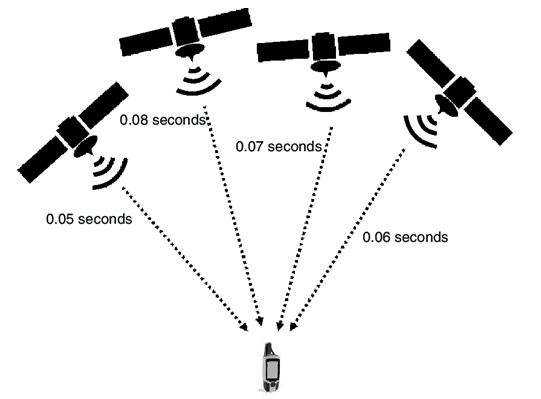
\includegraphics[scale=0.6]{./Figures/GPS}
\caption{GPS working scenario}
\label{fig:1}
 		\end{figure}
    
GPS does not work in indoor location because of no direct line of sight in indoor area. Here are some limitations:
\begin{itemize}
\item GPS signals carry waves at a frequency that is scattered by solid objects usually by buildings and walls.
\item Actually, satellites sent the signals that are not easily penetrate all kinds of barriers.
\item	When signal enters into the building, then it gets distorted due to construction material such as wood, bricks, cements etc because it serve as hindrance to the satellite signal.\cite{IP}

Hence, we can’t use outdoor localization technology like GPS in indoor environment.
\end{itemize}


\section{Indoor Localization Techniques}
Indoor localization techniques become popular day by day because it can provide ubiquitous location based services to people. Indoor positioning systems consist of a network of transmitters used for locating persons inside buildings. Here are the popular approaches: 
\subsection{Triangulation}
Triangulation technique uses the geometric properties of triangles in order to find the position of the object. In triangulation, AOA (Angle of Arrival)\cite{Sakpere2017ASS} technique is used to measure the angle and distance relative to two or multiple fixed points through the intersection of direction lines between the fixed points and then this information is used to calculate the position of transmitters which in turn describes the actual location of object.  In other words, position of target object is determined by the intersection of direction lines. Here is the illustration of this technique.
\begin{figure}[h]
  		\centering
    		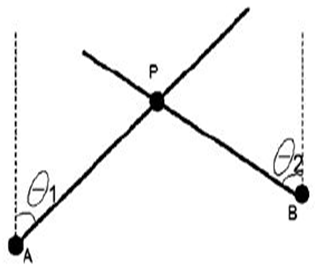
\includegraphics[scale=0.7]{./Figures/triangulation}
\caption{Illustration of triangulation technique}
\label{fig:2}
 		\end{figure}

\textbf{Drawbacks of Triangulation}

This method achieves good results outdoors but it gives weak results inside the building because the radio signals emitted by transmitters get attenuated by several obstacles hence it gives poor estimation of distance calculated. Moreover hardware requires special antennas for signal propagation and hardware requirement for the coverage of large area tends to be expensive and complex\cite{Sakpere2017ASS}. When the area becomes large with multiple reference points, accuracy will decreases due to some errors in the estimation of distance calculated.

\subsection{Trilateration}
Trilateration is also used to estimate the position of object using geometric properties of triangles. The position of target object is determined by TOA (Time of Arrival) and TDOA (Time difference of arrival) \cite{Sakpere2017ASS}. TOA is used to estimate the position of target object by calculating the time taken by a signal to reach the receiver from transmitter. TDOA is the improved version of TOA that considers the difference in TOA at two different receivers and then finds the relative position of transmitter based on the difference which further used to estimate the location of target object. This results in higher accuracy.

\textbf{Drawbacks of Trilateration}

The cost and complexity of hardware is high and it does not give good enough estimates in indoor area because of the inherent error of the distance measure calculations, hence most results have several meters of error\cite{cooper2016loco}. The accuracy is also affected by environmental conditions. In order to get good results both transmitter and receiver require precise clocks that should be synchronized. 

\subsection{Proximity}
Proximity technique is also used to estimate the location of target object. It requires a grid of antennas with known locations. When mobile device is detected by more than one antenna, then the antenna with the strongest signal is used to calculate its position. The position of target object (mobile device) is determined by using RSSI (Received Signal Strength Indication) to estimate the distance between mobile devices in order to get the position information of device.

\textbf{Drawbacks of Proximity}

Although proximity is applied on the systems using Bluetooth, IR but it requires calibration effort\cite{Sakpere2017ASS}. Also, we need larger spread of readers in order to achieve a reliable system but it increases system complexity and cost.

\subsection{Fingerprinting technique (Our Selected Approach)}
Fingerprinting technique is based on pattern matching technique. It is used to create signal strengths database that are based on the RSSI (Received Signal Strength Indication) values of various APs. These values are collected at different locations of an experimental area. These are called fingerprints, then by applying any machine learning approach we can train the model which further uses to predict the location of target user. Fingerprinting technique has a better positioning performance and accuracy as compared to the others and it doesn’t require any software or hardware modifications at transmitters end.

Here are the \textbf{indoor positioning technologies} which uses mostly any of method described above to predict location:

\textbf{1. Infrared (IR) positioning systems}

This system consists of a network of IR sensors that are linked by wires and then connected to a centralized server. Early badge system uses IR sensors for determining the position of object or people who is wearing badge.  Active Badge system uses IR sensors and TOA approach for estimating the location. Theses sensors are cheap and have good battery life. But the problem is that people have to wear the badge. This problem is solved by using IR thermal sensors\cite{Sakpere2017ASS} that uses the thermal rays emitted from human body for the prediction of location. Because we know that the temperature of human body is differs from room temperature.
\clearpage
\textbf{Drawbacks of IR positioning systems}

We need larger number of IR sensors to cover the large area which in turn increases system complexity and cost. Also these systems have limited accuracy. Thermal IR sensors also have major drawback that human body is not only the source of heat, there are also other heat sources like electronic devices and light bulbs that could affect the signals received from thermal IR sensors.

\textbf{2. Ultrasonic positioning systems}

This system contains ultrasonic sensors that emit ultrasonic signals which are used to estimate the location of object by measuring the TOF (Time of Flight) \cite{UPS}. The distance between transmitters and receiver is calculated by TOF and then this information is used to estimate the target position.

\textbf{Drawbacks of ultrasonic positioning systems}
This system is expensive and difficult to implement and maintain on larger area. Also, the ultrasound signals have low signal propagation speed when compared to speed of light\cite{Sakpere2017ASS}. It also affects by hindrances in indoor environment which in turn reduces its accuracy.

\textbf{3. Image based indoor localization}

It is a visual-based localization method. Early visual based methods require feature detection and matching that require huge computation and also it is affected by environmental conditions. There is a literature that implements this system by different approach. According to this research, firstly we need to build a database that contains collected images of experimental area. CNN (Convolution Neural Network) is used to train the model which is further used to predict the location of target object by inputting it the image of target location.\cite{image}

\textbf{Drawbacks of image based indoor localization}

Clearly, use of camera might be obtrusive for some users. Also time consuming effort is required to build the dataset and it also has scalability issue. Also, if we take image from different point of view which is not present in database, it might be possible that it would be predicted wrongly which in turn results the low accuracy. 

\textbf{4. Zigbee and capacitive sensors}

Zigbee sensors \cite{AAL} are also used for indoor location but they are very expensive and have medium scalability. Capacitive sensors \cite{AAL} are also used to estimate location by pressure sensing that detects the presence of a person but this system is very impractical to implement and deployment of sensors in floor is expensive.

\textbf{5. Wi-Fi based indoor localization}

In this, we can use either triangulation technique or fingerprinting technique for the estimation of the location of target user. But in triangulation, we require modification and special software to run on Wi-Fi base stations \cite{AAL}. But fingerprinting technique with Wi-Fi is a good approach for indoor localization because, we didn’t need any additional hardware for this system and we can use already deployed infrastructure. 

\textbf{Drawbacks of Wi-Fi based indoor localization}

Its main drawback is that it consumes more power. There are some spots where Wi-Fi access points would be difficult to power. There are some areas where Wi-Fi signals are not accessible. \cite{cooper2016loco}

\textbf{6. BLE beacons based indoor localization (our approach)}

After seeing the drawbacks of existing technologies, we decided to find the indoor location of a person using BLE beacons with fingerprinting technique, because it overcomes many drawbacks in existing systems, also they give better accuracy.  BLE beacons are Bluetooth low energy beacons. Classic Bluetooth consumes more power than BLE beacons and transmits to long ranges. BLE beacons are small in size, light weight and cheaper then Wi-Fi. BLE consumes less power than Wi-Fi. BLE beacons are usually battery powered, which are more flexible and easier deployed than sensors used by existing systems. BLE signals have higher sample rate than Wi-Fi signals. BLE consumes much less power because it transmits data over the small range \cite{BLEguide}. Bluetooth having version greater than 4.0 are BLE. BLE Beacon is a tiny device with a massively used for broadcasting of signals. It has unique ID (MAC Address). A BLE beacon has three major components:  ARM computer, a Bluetooth connectivity module and batteries for powering the entire circuit. The antenna is attached to the CPU of ARM computer. It broadcasts electromagnetic waves with specific length and frequency. Here is the internal circuitry of BLE beacon.

\begin{figure}[h]
  		\centering
    		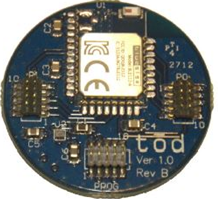
\includegraphics{./Figures/internalbeacon}
\caption{Internal circuitry of beacon}
\label{fig:3}
 		\end{figure}

Android phones with 4.3 and 4.3+ version support BLE \cite{BLEguide}, which makes it easy to implement. 
\\
\textbf{Conclusion}

As we can see there are many drawbacks in existing systems. In some systems, camera is required for indoor positioning which is obtrusive for some users. High cost and effort is required for the deployment of indoor localization infrastructure. Triangulation and trilateration proximity techniques require modifications at hardware end (Wi-Fi work stations) for the purpose of these techniques to work. These techniques also didn’t give satisfactory results in indoor environment due to the errors in distance measure calculations. Proximity technique also requires calibration effort and it is a costly technique to implement. Fingerprinting technique seems to be most suitable that’s why in our proposed system we use this technique. Most of the other existing systems have medium or low accuracy. In image based indoor localization, time consuming effort is required to build data sets. Wi-Fi fingerprinting is relatively better than other systems because of finding position by using already deployed infrastructure. But its main drawback is that it consumes more power. There are some spots where Wi-Fi access points would be difficult to power. So, after analyzing the drawbacks of existing technologies, we find out that BLE beacons with fingerprinting approach is most suitable because of various reasons that I have described above.

\section{Applications of GPS}
There are many applications of GPS which are as follows:
\begin{itemize}
\item Machinery and Information Technology for Bio Mass Production
\item Mobile Robot Sensors
\item Traffic sensing Technologies
\item Sensors and computing systems in Smart Clothing
\item Radio Navigation Systems
\end{itemize}
\textbf{Why we can’t use outdoor localization technology in indoor environment?}




\section{Problem Statement}
Whenever a visitor goes to university campus or visits a new place, he does not know about the specifications of that area i.e. what happens in that specific room or what courses have been taught in a particular and its nearby labs. So, we are developing a system which assists them in determining the textual and pictorial information of a particular area and its nearby locations. For this purpose, we first find the indoor location of a user by using BLE beacons and RSSI values, and then provide information to him automatically on his Android application. 